%% Los cap'itulos inician con \chapter{T'itulo}, estos aparecen numerados y
%% se incluyen en el 'indice general.
%%
%% Recuerda que aqu'i ya puedes escribir acentos como: 'a, 'e, 'i, etc.
%% La letra n con tilde es: 'n.

\chapter{Metodología}

Es sabido que tener información sobre la función de densidad o distribución de una variable aleatoria permite tener una completa descripción de la misma. Por este motivo es un problema fundamental de la Estadística obtener, a partir de la información proporcionada por una muestra,  buenas estimaciones de las funciones de densidad de una variable o vector aleatorio. 

En este sentido existen dos enfoques para abordar este problema. 

\begin{itemize}
	\item Un enfoque paramétrico: donde se considera que la función de densidad teórica pertenece a una familia de funciones de densidad $f_X(\vec{\theta})$ conocida, indexada por el vector de parámetros $\theta$. Bajo esta suposición estimar la función de densidad teórica se reduce a estimar el valor de los parámetros del modelo a partir de la información proporcionada por la muestra. Los métodos clásicos de estimación paramétrica son: Método de los Momentos y Método de Máxima Verosimilitud. En los últimos años el Método de LogCumulantes, que se basa en la transformada de Mellin, ha ganado interés por su buena performance.
	\item Un enfoque no paramétrico: donde no se hace ninguna suposición inicial sobre la familia de densidades a las que pertenece la función de densidad teórica, sino que trata de estimarla teniendo como única información los datos muestrales, imponiendo  solamente las condiciones necesarias para que dicha estimación sea una función de densidad.
\end{itemize}

El principal aporte de esta tesis es la propuesta de un nuevo método de estimación para los parámetros del modelo $\mathcal G_I^0$ con buenas propiedades que serán estudiadas a través del sesgo, del error cuadrático medio y de su capacidad para resistir presencia de datos atípicos, aún en el caso de muestras de pequeño y moderado tamaño. Este estimador surge de la minimización de distancias estocásticas entre la función de densidad teórica y una estimación no paramétrica de la función densidad subyacente utilizando núcleos asimétricos. 

En este capítulo describimos dos metodologías de estimación de la función de densidad: paramétrica y no paramétrica. Presentamos también la propuesta de este trabajo de tesis, el estimador de mínima distancia estocástica entre la función de densidad teórica del modelo $\mathcal{G}_I^0$ y una estimación no paramétrica de la función de densidad subyacente. Hacemos una discusión de diferentes distancias estocásticas estudiadas y diferentes núcleos utilizados para estimar la función de densidad.


\section{Estimación Paramétrica}

Esta metodología de estimación propone, a partir del conocimiento de la familia de densidades a la que pertenece la función de densidad teórica, estimar los parámetros que caracterizan dicha función de densidad a partir de datos muestrales. A continuación presentaremos métodos clásicos de estimación paramétrica.

\subsection{Método de los Momentos}
El Método de los Momentos (MOM) fue introducido por Karl Pearson en el año 1894 y se basa en la idea intuitiva de pensar que, si los datos muestrales provienen de una determinada función de densidad entonces los momentos muestrales deberían dar buenas estimaciones de los correspondientes momentos poblacionales. 

\begin{definition}
Si $X_1, \ldots, X_n$ es una muestra de variables aleatorias independientes e idénticamente distribuidas con función de densidad $f_{X;\theta}$, donde $\theta \in \mathbb{R}$ es el parámetro a estimar, y $g(x)$ una función de $\mathbb{R}$ en $\mathbb{R}$, el Método de los Momentos propone como estimador $\hat{\theta}_{mom}$ de $\theta$ aquel valor del parámetro que es solución de la ecuación  $\dfrac{1}{n} \sum_{i=1}^n g(X_i)=E_{\theta}(g(X_i)).$  
Si en cambio $X_i \sim f_{X;\vec{\theta}}$ con $\theta \in \Theta \subset \mathbb{R}^k$, entonces $\hat{\theta}_{mom}$ será el valor $\vec{\theta}$ que verifica el sistema de ecuaciones $\dfrac{1}{n} \sum_{i=1}^n g_s(X_i)=E_{\theta}(g_s(X_i))$ donde $s=1, \ldots k$ y $g_s(x)$ son $k$ funciones de $\mathbb{R}$ en $\mathbb{R}$.
\end{definition}


Obsevemos que si $g_s(x)=x^s$ la definición es consistente con la idea intuitiva mencionada anteriormente.
%Entonces, si $g(x)=x$ y el correspondiente momento muestral es $m_k=\dfrac{\sum_{i=1}^n X_i^k}{n}$. Entonces, si $X_1, \ldots X_n$ es una muestra de variables aleatorias independientes e idénticamente distribuidas 
%
%Recordemos que el $k$-ésimo momento muestral de una variable aleatoria $X$, tomado alrededor del origen, es $M_k=E(X^k)$.

El estimador por Momentos Fracionales ha sido estudiado en los últimos tiempos~\cite{Frery97,GambiniSC08,Khan2013}. En esta tesis se utilizarán los momentos de orden $1$ y de orden $\frac{1}{2}$ porque mostraron una mejor performance a la hora de estimar los parámetros de la distribución $\mathcal G_I^0$ respecto de los momentos de orden $1$ y de orden $2$.

Las ecuaciones de momento de orden $1$ y de orden $\frac{1}{2}$ para estimar los parámetros de la distribución $\mathcal G_I^0$ son:

\begin{align}
\overline{X}=&\dfrac{\gamma}{-\alpha - 1} \\
\nonumber \\ 
\dfrac{\sum_{i=1}^n X_i^{1/2}}{n}=&\dfrac{\gamma^{1/2}}{L^{1/2}}\dfrac{\Gamma(-\alpha - 1/2)}{\Gamma(-\alpha)}\dfrac{\Gamma(L+ 1/2)}{\Gamma(L)}.
\end{align}


\subsection{Método de Máxima Verosimilitud}

 El Método de Máxima Verosimilitud fue popularizado por R. Fisher entre 1912 y 1922. Sin embargo este método había sido utilizado antes por Gauss, Laplace entre otros investigadores. La idea del método consiste en, dada una muestra, estimar los parámetros de la distribución que maximice la probabilidad de que haya salido esa muestra. Este estimador tiene muy buenas propiedades asintóticas, además de ser consistente es asintóticamente normal y eficiente bajo condiciones generales.

\begin{definition}
Si $X_1, \ldots, X_n$ es una muestra de variables aleatorias independientes e idénticamente distribuidas con función de densidad $f_{X;\vec{\theta}}$  con $\vec{\theta} \in \Theta \subset \mathbb{R}^k$, diremos que $\widehat{\vec{\theta}}_{MV}$ es el estimador de máxima verosimilitud de $\vec{\theta}$ si verifica que 
\begin{align}
\widehat{\vec{\theta}}_{{\text{\tiny{MV}}}}=\arg\max_{\vec{\theta \in \Theta}} L(\vec{\theta}/\vec{X}=\vec{x})
\end{align}
siendo $L(\vec{\theta}/\vec{X}=\vec{x})$ la función de verosimilitud, que es la función de densidad conjunta del vector aleatorio $\vec{X}$ mirada como función del vector de parámetros $\vec{\theta}$, sabiendo que salió la muestra $\vec{x}$.
\end{definition}

El parámetro $\gamma$ en la distribución $\mathcal{G}_I^0$  es proporcional al brillo y es un parámetro de escala. Con el fin de reducir nuestro análisis a un solo parámetro, y con el propósito de hacer los resultados comparables, basamos nuestro análisis en la condición $E(Z)=1$ que vincula la textura con el brillo. Esta condición nos da una relación entre $\gamma$ y $\alpha$ que es la siguiente:
\begin{align}
\label{gama*}
\gamma=-\alpha-1. 
\end{align}
A este valor de $\gamma$ lo llamaremos $\gamma^*$.

Entonces, si $Z_1,\ldots Z_n$ una muestra de variables aleatorias independientes e idénticamente distribuidas donde $Z_i \sim f_{\mathcal G_I^0(\alpha,\gamma)}(z)$,  el logaritmo de la función de verosimilitud bajo la condición~\eqref{gama*} es:

\begin{align}
\nonumber \log(L(\alpha)/\vec{Z}=\vec{z})&=n(L \log(L)+log(\Gamma(L-\alpha))-\log(\Gamma(L))-\log(\Gamma(-\alpha))-\alpha \log(-\alpha-1))\\
& + (L-1) \sum_{i=1}^n \log(z_i))-(L-\alpha) \sum_{i=1}^n(\log(-\alpha-1+z_i L))).
\end{align}

%\begin{align}
%\nonumber \log(L(\alpha,\gamma)/\vec{Z}=\vec{z})&=n(L \log(L)+log(\Gamma(L-\alpha))-\log(\Gamma(L))-\log(\Gamma(-\alpha))-\alpha \log(\gamma))\\
% & + (L-1) \sum_{i=1}^n \log(z_i))-(L-\alpha) \sum_{i=1}^n(\log(\gamma+z_i L))).
%\end{align}

Por lo tanto, el estimador de máxima verosimilitud (ML) del parámetro de textura es:
\begin{align}
\widehat{\alpha}_{{\text{\tiny{MV}}}}=\arg\max_{\alpha} \log(L(\alpha)/\vec{Z}=\vec{z}).
\end{align}

Algunos autores evaluaron la performance para el estimador de máxima verosimilitud del parámetro de textura del modelo  $\mathcal G_I^0$. Vasconcellos et al.~\cite{VasconcellosFrerySilva:CompStat} cuantificaron el sesgo de este estimador y propusieron una corrección de segundo orden de acuerdo a~\cite{cox1968}. Cribari-Neto et al.~\cite{CribariFrerySilva:CSDA} desarrollaron una corrección del sesgo de $\widehat{\alpha}_{\text{{\text{\tiny{ML}}}}}$ del modelo $\mathcal G^0$ para datos de amplitud usando técnicas de remuestreo a expensas de un alto costo computacional.

En la figura~\ref{MV} se muestra el gráfico del logaritmo de la función de verosimilitud en función de $\alpha$, para distintos tamaños de muestra $n$ y para dos valores del parámetro de textura: $\alpha=-1.5$ y $\alpha=-5$ para el caso de $L=3$. Se puede observar que, para zonas extremadamente texturadas la función de verosimilitud muestra claramente un máximo. Sin embargo, para el caso de zonas texturadas esta función es bastante plana, incluso podría ser monótona dependiendo de la muestra. Esto puede originar problemas numéricos al momento de encontrar el máximo.  

\begin{figure}[hbt]
	\centering    
	\label{MV}
	\subfigure[$\alpha=-1.5$]{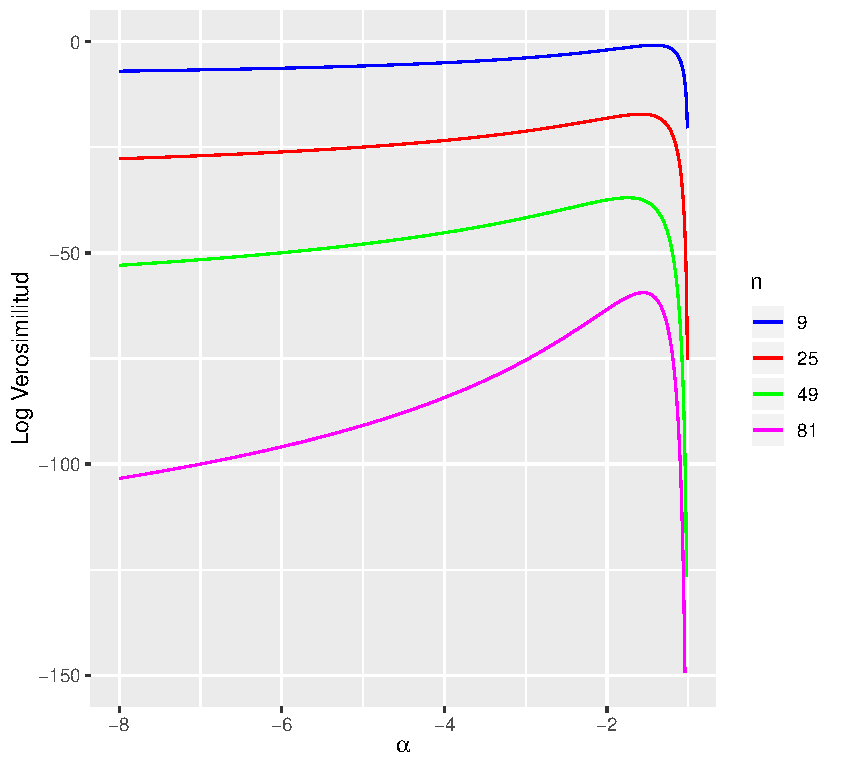
\includegraphics[scale=0.5]{../../Figures/Tesis/Capitulo4/Verosimilitud1punto5_2.pdf}}
	\subfigure[$\alpha=-5$]{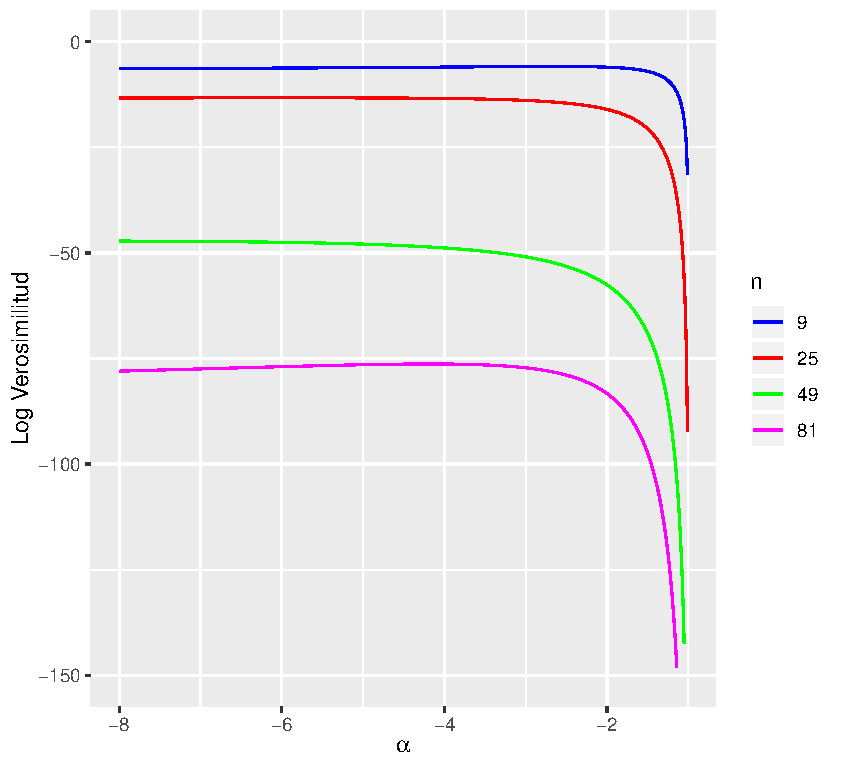
\includegraphics[scale=0.5]{../../Figures/Tesis/Capitulo4/Verosimilitud-5_2.pdf}}
	\caption{Función de verosimilitud para $L=3$}
\end{figure}

También se podría encontrar $\widehat{\alpha}_{{\text{\tiny{MV}}}}$ como la solución de la siguiente ecuación no lineal.

\begin{align}
\label{rootML}
\Psi^0(-\widehat{\alpha}_{{\text{\tiny{MV}}}})-\Psi^0(L-\widehat{\alpha}_{{\text{\tiny{MV}}}})-\log(-1-\widehat{\alpha}_{{\text{\tiny{MV}}}})+{} \nonumber\\
\frac{\widehat{\alpha}_{{\text{\tiny{MV}}}}}{-1-\widehat{\alpha}_{{\text{\tiny{MV}}}}}+
\frac{1}{n}\sum_{i=1}^n{\log(-1-\widehat{\alpha}_{{\text{\tiny{MV}}}}+Lz_i)}-{}
\nonumber
\\ \frac{\widehat{\alpha}_{{\text{\tiny{MV}}}}-L}{n}\sum_{i=1}^n \frac1{-1-\widehat{\alpha}_{{\text{\tiny{MV}}}}+Lz_i}= 0, 
\end{align}
donde $\Psi^0(\cdot)$ es la función digamma. Este sistema no tiene una solución analítica cerrada, por lo tanto es necesario la utilización de rutinas numéricas para encontrar dicha solución que puede incluso no existir.

\subsection{Log Momentos y Log Cumulantes}

Es conocida la relación que existe entre los momentos y la función característica de una variable aleatoria con la transformada de Fourier de su función de densidad. 

\begin{definition}
Si $X$ es una variable aleatoria continua con función de densidad $f_X(x)$, la función característica $\phi_X: \mathbb{R} \rightarrow \mathbb{C}$ se define como 
\begin{align}
\phi_X(t)=E(e^{itX})=\int_{-\infty}^{\infty} e^{itx} f_X(x) dx = \mathcal{F}\{f_X\}(t),
\label{fi}
\end{align}
siendo $\mathcal{F}\{f_X\}$ la transformada de Fourier de $f_X$.
\end{definition}

Cuando los momentos de orden $n$ de una variable aleatoria existen, es decir, cuando $E(X^k)< \infty$, se puede apelar a la relación~\eqref{fi} para calcular dichos momentos. Entonces

\begin{align}
\phi_X^{(k)}(0)=i^k E(X^k)
\label{fi}
\end{align}
con $\phi_X^{(k)}$ la derivada de orden $k$ de $\phi_X$ evaluada en $t=0$. Luego, los momentos de orden $k$ se pueden definir como 

\begin{align}
\label{MomentosPrimerTipo}
m_k=E(X^k)=i^{-k} \phi_X^{(k)}(t)\big\arrowvert _{t=0}
\end{align}

Si llamamos $\psi_X=\log(\phi_X)$, los cumulantes de orden $k$ se definen como 

\begin{align}
\label{CumulantePrimerTipo}
\kappa_k=i^{-k} \psi_X^{(k)}\big\arrowvert _{t=0}
\end{align}

Nicolas et al.~\cite{nicolas2002} proponen utilizar la transformada de Mellin en lugar de la transformada de Fourier en~\eqref{fi}, para el caso donde la función de densidad $f_X$ de la variable aleatoria $X$ tiene soporte positivo. De esta manera surgen nuevas características para la variable aleatoria que son los Log Momentos (MomL) y los Log Cumulantes (MomLC). Los autores proponen llamar a esta metodología Estadísticas de Segundo Tipo. Entonces, análogamente a la metodología descripta en~\ref{fi}, definen:

\begin{itemize}
\item Primer función característica de segundo tipo.
	\begin{align}
	\Phi_X(s)=\int_{0}^{\infty} x^{s-1} f_X(x) dx = \mathcal{M}\{f_X\}(s)
	\label{PrimerFuncionCaract}
	\end{align}
\item Momentos de segundo tipo.
	\begin{align}
	\label{MomentoSegundoTipo}
	\tilde{m}_k=\Phi_X^{(k)}(s) \big\arrowvert _{s=1}
	\end{align}


	Una propiedad interesante que cumplen las derivadas de orden $k$ de la transformada de Mellin de una función $h(x)$ es $\mathcal{M}\{\ln(x)^k h(x)\}(s)=\mathcal{M}^{(k)}\{h(x)\}(s)$. Entonces, aplicando esta propiedad a~\eqref{PrimerFuncionCaract} y~\eqref{MomentoSegundoTipo}, y considerando $h=f_X$ se obtiene:

	\begin{align}
	\label{MomL}
	\nonumber \tilde{m}_k&=\Phi_X^{(k)}(s) \big\arrowvert _{s=1} =\mathcal{M}^{(k)}\{f(x)\}(s) =\mathcal{M}\{f(x) \log(x)^k\}(s)\big\arrowvert _{s=1}          \\
 	        &=\int_{0}^{\infty} \log(x)^k f_X(x) dx 
	\end{align}

	Esta última ecuación sugiere llamar a los momentos de segundo tipo como \textit{Log Momentos} (MomL).
	
\item Segunda función característica de segundo tipo.

      Manteniendo la analogía con las estadísticas de primer tipo, Nicolas et al.~\cite{nicolas2002} definen la \textit{Segunda función característica de segundo tipo} como
      \begin{align}
      \label{Sgunda Psi}
      \Psi_X(s)=\log(\Phi)(s)
      \end{align}
      
\item Cumulantes de segundo tipo.

	  Las derivadas de orden $k$ de la segunda función característica de segundo tipo, evaluada en $s=1$, se definen como los cumulantes de segundo tipo. Entonces,
	  \begin{align}
	  \label{CumulanteSegundoTipo}
	  \tilde{\kappa}_k=\Psi_X^{(k)}\big\arrowvert _{s=1}
	  \end{align}
	  
Como en el caso de MomL, los cumulantes de segundo tipo se llamarán \textit{Log Cumulantes} (MomLC).
\end{itemize}

Para el caso donde $f_X(u) = \mathcal{G}_I^0(u)$ se obtiene:
	\begin{align}
	\Phi_x(s) &= \dfrac{\left(\frac{L}{\gamma}\right)^{1-s}\Gamma(-1+L+s)\Gamma(1-s-\alpha)}{\Gamma(L)\Gamma(-\alpha)} \\
	\vspace{1cm}
	\nonumber \widetilde{m}_1 &=  \frac{d \Phi_x(s)}{ds } \big\arrowvert _{s=1}\\
					& = -\log\left(\frac{L}{\gamma}\right) + \Psi^0(L) - \Psi^0(-\alpha).
	\end{align}

Usando los desarrollos presentados en Tison et al.~\cite{Tison2004} tenemos que $\widetilde{k}_1 = \widetilde{m_1}$. Por lo tanto 
\begin{align}
\label{MomLC}
\widetilde{k}_1 =   -\log \left(\frac{L}{\gamma}\right) + \Psi^0(L) - \Psi^0(-\alpha).
\end{align}

Además, si $Z_1,\ldots,Z_n$ es una muestra de variables aleatorias independientes e idénticamente distribuidas donde $Z_i \sim \mathcal{G}_I^0$, usando\eqref{MomL} tenemos que MomLC es
\begin{align}
\label{EstimadorMomLC}
\widehat{\widetilde{k}}_1 =\dfrac{1}{n} \sum_{i=1}^k\log z_i
\end{align}

Asumiendo que vale la relación~\eqref{gama*}, $\gamma^*=-\alpha-1$, el estimador Log Cumulante del parámetro de textura $\alpha$ de la distribución $\mathcal{G}_I^0$, que lo llamaremos $\alpha_{\text{\tiny{LC}}}$, es la solución de la ecuación    
\begin{align}
\widehat{\widetilde{k}}_1 =   -\log \left(\frac{L}{1-\widehat\alpha_{\text{\tiny{LC}}}}\right) + \Psi^0(L) - \Psi^0(-\widehat\alpha_{\text{\tiny{LC}}})
\end{align}
es decir, la solución de la ecuación
\begin{equation} \label{eq:logm}
\frac{1}{n} \sum_{i=1}^n\log (z_i) =   -\log \left(\frac{L}{1-\widehat\alpha_{\text{\tiny{LC}}}}\right) + \Psi^0(L) + \Psi^0(-\widehat\alpha_{\text{\tiny{LC}}}).
\end{equation}


\section{Estimación No Paramétrica}

Como mencionamos anteriormente, otra posibilidad para estimar los parámetros de un modelo es la estimación no paramétrica. Esta metodología de estimación  no determina a priori ningún modelo para la distribución de la variable aleatoria de interés, y propone estimadores de la función de densidad sin más límites que los necesarios para que estos estimadores cumplan con las condiciones de ser una función de densidad.

\subsection{Estimadores de Mínima Distancia}
\subsection{Distancias Estocásticas}
\subsection{Núcleos asimétricos}

